\documentclass[preprint,showkeys,nofootinbib]{revtex4-1}


% linking references
\usepackage{hyperref}
\hypersetup{
  breaklinks=true,
  colorlinks=true,
  linkcolor=blue,
  urlcolor=cyan,
}


% general physics / math packages and commands
\usepackage{physics,amsmath,amssymb,braket,dsfont}
\renewcommand{\t}{\text} % text in math mode
\newcommand{\f}{\dfrac} % shorthand for fractions
\newcommand{\p}[1]{\left(#1\right)} % parenthesis
\renewcommand{\sp}[1]{\left[#1\right]} % square parenthesis
\renewcommand{\set}[1]{\left\{#1\right\}} % curly parenthesis
\newcommand{\bk}{\braket} % shorthand for braket

\renewcommand{\d}{\text{d}}
\newcommand{\g}{\text{g}}
\newcommand{\e}{\text{e}}
\newcommand{\x}{\text{x}}
\newcommand{\y}{\text{y}}
\newcommand{\z}{\text{z}}

\renewcommand{\c}{\hat{c}}
\newcommand{\n}{\hat{n}}

\newcommand{\A}{\mathcal{A}}
\newcommand{\B}{\mathcal{B}}
\newcommand{\D}{\mathcal{D}}
\newcommand{\E}{\mathcal{E}}
\newcommand{\G}{\mathcal{G}}
\renewcommand{\H}{\mathcal{H}}
\newcommand{\I}{\mathcal{I}}
\newcommand{\K}{\mathcal{K}}
\renewcommand{\L}{\mathcal{L}}
\newcommand{\M}{\mathcal{M}}
\newcommand{\N}{\mathcal{N}}
\renewcommand{\O}{\mathcal{O}}
\renewcommand{\P}{\mathcal{P}}
\newcommand{\Q}{\mathcal{Q}}
\renewcommand{\S}{\mathcal{S}}
\newcommand{\U}{\mathcal{U}}

\newcommand{\1}{\mathds{1}}

\newcommand{\mA}{m_{\text{A}}} % symbol for the mass of an atom


% "left vector" arrow; requires tikz package
\newcommand{\lvec}[1]
{\reflectbox{\ensuremath{\vec{\reflectbox{\ensuremath{#1}}}}}}


% figures
\usepackage{graphicx} % for figures
\usepackage{grffile} % help latex properly identify figure extensions
\graphicspath{{./figures/}} % set path for all figures
\usepackage[caption=false]{subfig} % subfigures (via \subfloat[]{})


% inline lists
\usepackage[inline]{enumitem}


% for feynman diagrams
\usepackage{tikz,tikz-feynman}
\tikzset{
  baseline = (current bounding box.center)
}
\tikzfeynmanset{
  compat = 1.1.0,
  every feynman = {/tikzfeynman/small}
}
\newcommand{\shrink}[1]{\scalebox{0.8}{#1}} % for smaller diagrams


% color definitions (used in a figure)
\usepackage{xcolor}
\definecolor{lightblue}{RGB}{31,119,180}
\definecolor{orange}{RGB}{255,127,14}
\definecolor{green}{RGB}{44,160,44}
\definecolor{lightred}{RGB}{214,39,40}

% proper coloring inside math environment
\makeatletter
\def\mathcolor#1#{\@mathcolor{#1}}
\def\@mathcolor#1#2#3{
  \protect\leavevmode
  \begingroup
    \color#1{#2}#3
  \endgroup
}
\makeatother
\newcommand{\bmu}{\mathcolor{lightblue}{\mu}}
\newcommand{\onu}{\mathcolor{orange}{\nu}}
\newcommand{\grho}{\mathcolor{green}{\rho}}
\newcommand{\re}{\mathcolor{lightred}{\text{e}}}


% leave a note in the text, visible in the compiled document
\newcommand{\note}[1]{\textcolor{red}{#1}}

% for strikeout text
% normalem included to prevent underlining titles in the bibliography
\usepackage[normalem]{ulem}


\newcommand{\blue}[1]{\textcolor{blue}{#1}}
\newcommand{\red}[1]{\textcolor{red}{#1}}
\newcommand{\green}[1]{\textcolor{green}{#1}}

% for numbering points in response to referees
\newcounter{point}
\newcommand{\step}{\stepcounter{point}\setcounter{enumi}{0}}


\begin{document}

Dear editors,

In this document, we summarize all revisions made to our manuscript
since the previous version, i.e.~the version submitted after the first
round of review.  Excerpts from the previous version of our manuscript
(i.e.~submitted after the first round of review) are written in
\red{red}, and excerpts from the final version of our manuscript is
written in \green{green}.  All page, line, equation, and reference
numbers generally refer to those from the previous version of our
manuscript.

\begin{enumerate}
\item Referee 1 pointed out an error in section III.D of our
  manuscript.  We have fixed this error, and rearranged the text in
  section III.D to improve readability in light of these changes.
  Specifically, we have we have replaced the following text (page 19,
  line 14):

  \red{To leading order in the coupling constants, the renormalization
    condition in (16) implies that
    \begin{align}
      \shrink{
        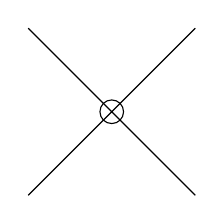
\begin{tikzpicture}
          \begin{feynman}
            \vertex[crossed dot] (v) {};
            \vertex[above left = of v] (f1);
            \vertex[below left = of v] (f2);
            \vertex[above right = of v] (f3);
            \vertex[below right = of v] (f4);
            \diagram* {
              (f1) -- (v),
              (f2) -- (v),
              (v) -- (f3),
              (v) -- (f4), };
          \end{feynman}
        \end{tikzpicture}}
      = \shrink{
        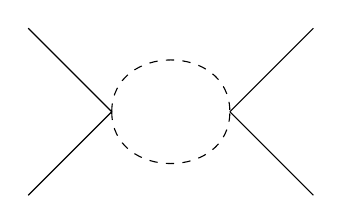
\begin{tikzpicture}
          \begin{feynman}
            \vertex (v1);
            \vertex[right = of v1] (v2);
            \vertex[above left = of v1] (f1);
            \vertex[below left = of v1] (f2);
            \vertex[above right = of v2] (f3);
            \vertex[below right = of v2] (f4);
            \diagram* {
              (f1) -- (v1) --[half left, scalar] (v2) -- (f3),
              (f2) -- (v1) --[half right, scalar] (v2) -- (f4), };
          \end{feynman}
        \end{tikzpicture}},
      \tag{25}
    \end{align}
    which means that the sum over all counter-term diagrams in (24) is
    \begin{align}
      \shrink{
        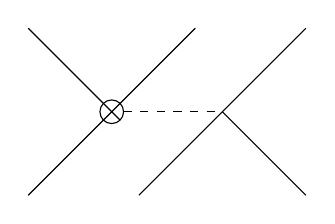
\begin{tikzpicture}
          \begin{feynman}
            \vertex[crossed dot] (v1) {};
            \vertex[right = 4em of v1] (v2);
            \vertex[above left = of v1] (f1);
            \vertex[below left = of v1] (f2);
            \vertex[above right = of v1] (f3);
            \vertex[below left = of v2] (f4);
            \vertex[below right = of v2] (f5);
            \vertex[above right = of v2] (f6);
            \diagram* {
              (f1) -- (v1) -- (f3),
              (f2) -- (v1) --[scalar] (v2),
              (f4) -- (v2) -- (f5),
              (v2) -- (f6), };
          \end{feynman}
        \end{tikzpicture}}
      = \shrink{
        \begin{tikzpicture}
          \begin{feynman}
            \vertex (v1);
            \vertex[right = of v1] (v2);
            \vertex[below right = of v2] (v3);
            \vertex[above left = of v1] (f1);
            \vertex[below left = of v1] (f2);
            \vertex[below left = of v3] (f3);
            \vertex[above right = of v2] (f4);
            \vertex[above right = of v3] (f5);
            \vertex[below right = of v3] (f6);
            \diagram* {
              (f1) -- (v1) --[half left, scalar] (v2) -- (f4),
              (f2) -- (v1) --[half right, scalar] (v2)
              --[scalar] (v3) -- (f5),
              (f3) -- (v3) -- (f6), };
          \end{feynman}
        \end{tikzpicture}}.
      \tag{26}
    \end{align}
    The net contribution of the these counter-term diagrams together
    with the two-particle-loop diagrams in (23) is therefore
    \begin{multline}
      - \shrink{
        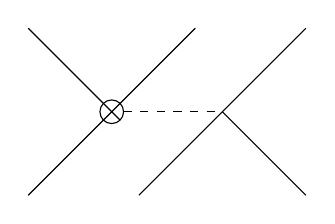
\begin{tikzpicture}
          \begin{feynman}
            \vertex[crossed dot] (v1) {};
            \vertex[right = 4em of v1] (v2);
            \vertex[above left = of v1] (f1);
            \vertex[below left = of v1] (f2);
            \vertex[above right = of v1] (f3);
            \vertex[below left = of v2] (f4);
            \vertex[below right = of v2] (f5);
            \vertex[above right = of v2] (f6);
            \diagram* {
              (f1) -- (v1) -- (f3),
              (f2) -- (v1) --[scalar] (v2),
              (f4) -- (v2) -- (f5),
              (v2) -- (f6), };
          \end{feynman}
        \end{tikzpicture}}
      + \shrink{
        \begin{tikzpicture}
          \begin{feynman}
            \vertex (v1);
            \vertex[right = of v1] (v2);
            \vertex[below right = of v2] (v3);
            \vertex[above left = of v1] (f1);
            \vertex[below left = of v1] (f2);
            \vertex[below left = of v3] (f3);
            \vertex[above right = of v2] (f4);
            \vertex[above right = of v3] (f5);
            \vertex[below right = of v3] (f6);
            \diagram* {
              (f1) -- (v1) --[half left, scalar] (v2) -- (f4),
              (f2) -- (v1) --[half right, scalar] (v2)
              --[scalar] (v3) -- (f5),
              (f3) -- (v3) -- (f6), };
          \end{feynman}
        \end{tikzpicture}}
      - \f12 \shrink{
        \begin{tikzpicture}
          \begin{feynman}
            \vertex (v1);
            \vertex[right = of v1] (v2);
            \vertex[below right = of v2] (v3);
            \vertex[above left = of v1] (f1);
            \vertex[below left = of v1] (f2);
            \vertex[below left = of v3] (f3);
            \vertex[above right = of v2] (f4);
            \vertex[above right = of v3] (f5);
            \vertex[below right = of v3] (f6);
            \diagram* {
              (f1) -- (v1) --[half left, scalar] (v2) -- (f4),
              (f2) -- (v1) --[half right, scalar] (v2)
              -- (v3) -- (f5),
              (f3) -- (v3) -- (f6), };
          \end{feynman}
        \end{tikzpicture}}
      - \f12 \shrink{
        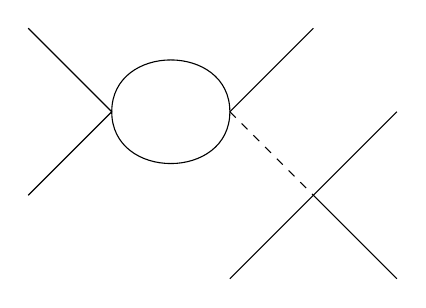
\begin{tikzpicture}
          \begin{feynman}
            \vertex (v1);
            \vertex[right = of v1] (v2);
            \vertex[below right = of v2] (v3);
            \vertex[above left = of v1] (f1);
            \vertex[below left = of v1] (f2);
            \vertex[below left = of v3] (f3);
            \vertex[above right = of v2] (f4);
            \vertex[above right = of v3] (f5);
            \vertex[below right = of v3] (f6);
            \diagram* {
              (f1) -- (v1) --[half left] (v2) -- (f4),
              (f2) -- (v1) --[half right] (v2)
              --[scalar] (v3) -- (f5),
              (f3) -- (v3) -- (f6), };
          \end{feynman}
        \end{tikzpicture}} \\
      = - \f12 \shrink{
        \begin{tikzpicture}
          \begin{feynman}
            \vertex (v1);
            \vertex[right = of v1] (v2);
            \vertex[below right = of v2] (v3);
            \vertex[above left = of v1] (f1);
            \vertex[below left = of v1] (f2);
            \vertex[below left = of v3] (f3);
            \vertex[above right = of v2] (f4);
            \vertex[above right = of v3] (f5);
            \vertex[below right = of v3] (f6);
            \diagram* {
              (f1) -- (v1) --[half left, scalar] (v2) -- (f4),
              (f2) -- (v1) --[half right, scalar] (v2)
              -- (v3) -- (f5),
              (f3) -- (v3) -- (f6), };
          \end{feynman}
        \end{tikzpicture}}
      - \f12 \shrink{
        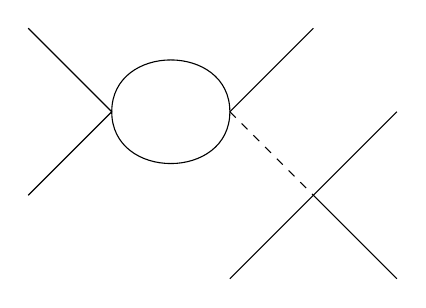
\begin{tikzpicture}
          \begin{feynman}
            \vertex (v1);
            \vertex[right = of v1] (v2);
            \vertex[below right = of v2] (v3);
            \vertex[above left = of v1] (f1);
            \vertex[below left = of v1] (f2);
            \vertex[below left = of v3] (f3);
            \vertex[above right = of v2] (f4);
            \vertex[above right = of v3] (f5);
            \vertex[below right = of v3] (f6);
            \diagram* {
              (f1) -- (v1) --[half left] (v2) -- (f4),
              (f2) -- (v1) --[half right] (v2)
              --[scalar] (v3) -- (f5),
              (f3) -- (v3) -- (f6), };
          \end{feynman}
        \end{tikzpicture}}.
      \tag{27}
    \end{multline}
    An identical cancellation occurs for the mirror images of the
    diagrams in (23) and (24), which results in a contribution to the
    effective Hamiltonian that is equal to (27).  The contribution
    from the three-particle-loop diagrams in (22) is
    \begin{multline}
      \shrink{
        \begin{tikzpicture}
          \begin{feynman}
            \vertex (v1);
            \vertex[below right = of v1] (v2);
            \vertex[above right = of v2] (v3);
            \vertex[above left = of v1] (f1);
            \vertex[left = of v1] (f2);
            \vertex[below left = of v2] (f3);
            \vertex[above right = of v3] (f4);
            \vertex[right = of v3] (f5);
            \vertex[below right = of v2] (f6);
            \diagram* {
              (f1) -- (v1) --[scalar] (v3) -- (f4),
              (f2) -- (v1) --[scalar] (v2) --[scalar] (v3) -- (f5),
              (f3) -- (v2) -- (f6), };
          \end{feynman}
        \end{tikzpicture}}
      - \f12 \shrink{
        \begin{tikzpicture}
          \begin{feynman}
            \vertex (v1);
            \vertex[below right = of v1] (v2);
            \vertex[above right = of v2] (v3);
            \vertex[above left = of v1] (f1);
            \vertex[left = of v1] (f2);
            \vertex[below left = of v2] (f3);
            \vertex[above right = of v3] (f4);
            \vertex[right = of v3] (f5);
            \vertex[below right = of v2] (f6);
            \diagram* {
              (f1) -- (v1) -- (v3) -- (f4),
              (f2) -- (v1) --[scalar] (v2) -- (v3) -- (f5),
              (f3) -- (v2) -- (f6), };
          \end{feynman}
        \end{tikzpicture}}
      - \f12 \shrink{
        \begin{tikzpicture}
          \begin{feynman}
            \vertex (v1);
            \vertex[below right = of v1] (v2);
            \vertex[above right = of v2] (v3);
            \vertex[above left = of v1] (f1);
            \vertex[left = of v1] (f2);
            \vertex[below left = of v2] (f3);
            \vertex[above right = of v3] (f4);
            \vertex[right = of v3] (f5);
            \vertex[below right = of v2] (f6);
            \diagram* {
              (f1) -- (v1) -- (v3) -- (f4),
              (f2) -- (v1) -- (v2) --[scalar] (v3) -- (f5),
              (f3) -- (v2) -- (f6), };
          \end{feynman}
        \end{tikzpicture}} \\
      = \shrink{
        \begin{tikzpicture}
          \begin{feynman}
            \vertex (v1);
            \vertex[below right = of v1] (v2);
            \vertex[above right = of v2] (v3);
            \vertex[above left = of v1] (f1);
            \vertex[left = of v1] (f2);
            \vertex[below left = of v2] (f3);
            \vertex[above right = of v3] (f4);
            \vertex[right = of v3] (f5);
            \vertex[below right = of v2] (f6);
            \diagram* {
              (f1) -- (v1) --[scalar] (v3) -- (f4),
              (f2) -- (v1) --[scalar] (v2) --[scalar] (v3) -- (f5),
              (f3) -- (v2) -- (f6), };
          \end{feynman}
        \end{tikzpicture}}
      - \shrink{
        \begin{tikzpicture}
          \begin{feynman}
            \vertex (v1);
            \vertex[below right = of v1] (v2);
            \vertex[above right = of v2] (v3);
            \vertex[above left = of v1] (f1);
            \vertex[left = of v1] (f2);
            \vertex[below left = of v2] (f3);
            \vertex[above right = of v3] (f4);
            \vertex[right = of v3] (f5);
            \vertex[below right = of v2] (f6);
            \diagram* {
              (f1) -- (v1) -- (v3) -- (f4),
              (f2) -- (v1) --[scalar] (v2) -- (v3) -- (f5),
              (f3) -- (v2) -- (f6), };
          \end{feynman}
        \end{tikzpicture}}.
      \tag{28}
    \end{multline}
    The third-order three-body interaction Hamiltonian is therefore
    \begin{align}
      H_3^{(3)} &= \shrink{
        \begin{tikzpicture}
          \begin{feynman}
            \vertex (v1);
            \vertex[below right = of v1] (v2);
            \vertex[above right = of v2] (v3);
            \vertex[above left = of v1] (f1);
            \vertex[left = of v1] (f2);
            \vertex[below left = of v2] (f3);
            \vertex[above right = of v3] (f4);
            \vertex[right = of v3] (f5);
            \vertex[below right = of v2] (f6);
            \diagram* {
              (f1) -- (v1) --[scalar] (v3) -- (f4),
              (f2) -- (v1) --[scalar] (v2) --[scalar] (v3) -- (f5),
              (f3) -- (v2) -- (f6), };
          \end{feynman}
        \end{tikzpicture}}
      - \shrink{
        \begin{tikzpicture}
          \begin{feynman}
            \vertex (v1);
            \vertex[below right = of v1] (v2);
            \vertex[above right = of v2] (v3);
            \vertex[above left = of v1] (f1);
            \vertex[left = of v1] (f2);
            \vertex[below left = of v2] (f3);
            \vertex[above right = of v3] (f4);
            \vertex[right = of v3] (f5);
            \vertex[below right = of v2] (f6);
            \diagram* {
              (f1) -- (v1) -- (v3) -- (f4),
              (f2) -- (v1) --[scalar] (v2) -- (v3) -- (f5),
              (f3) -- (v2) -- (f6), };
          \end{feynman}
        \end{tikzpicture}}
       - \shrink{
        \begin{tikzpicture}
          \begin{feynman}
            \vertex (v1);
            \vertex[right = of v1] (v2);
            \vertex[below right = of v2] (v3);
            \vertex[above left = of v1] (f1);
            \vertex[below left = of v1] (f2);
            \vertex[below left = of v3] (f3);
            \vertex[above right = of v2] (f4);
            \vertex[above right = of v3] (f5);
            \vertex[below right = of v3] (f6);
            \diagram* {
              (f1) -- (v1) --[half left, scalar] (v2) -- (f4),
              (f2) -- (v1) --[half right, scalar] (v2) -- (v3)
              -- (f5),
              (f3) -- (v3) -- (f6), };
          \end{feynman}
        \end{tikzpicture}}
      - \shrink{
        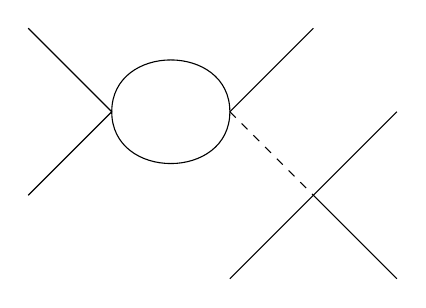
\begin{tikzpicture}
          \begin{feynman}
            \vertex (v1);
            \vertex[right = of v1] (v2);
            \vertex[below right = of v2] (v3);
            \vertex[above left = of v1] (f1);
            \vertex[below left = of v1] (f2);
            \vertex[below left = of v3] (f3);
            \vertex[above right = of v2] (f4);
            \vertex[above right = of v3] (f5);
            \vertex[below right = of v3] (f6);
            \diagram* {
              (f1) -- (v1) --[half left] (v2) -- (f4),
              (f2) -- (v1) --[half right] (v2) --[scalar] (v3)
              -- (f5),
              (f3) -- (v3) -- (f6), };
          \end{feynman}
        \end{tikzpicture}} \nonumber \\[1em]
      &= \p{\alpha_3^{(3)} - \alpha_5^{(3)}} \H_{3,1}^{(3)}
      - \p{\alpha_{4,3}^{(3)} + \alpha_5^{(3)}} \H_{3,2}^{(3)},
      \tag{29}
    \end{align}
    where, letting $E_{mn}\equiv E_m+E_n$,
    \begin{align}
      \alpha_3^{(3)} \equiv \sum_{\substack{\ell+m>0\\\ell+n>0}}
      \f{K_{\ell m} K^m_n K_{\ell n}}{E_{\ell m} E_{\ell n}},
      &&
      \alpha_{4,3}^{(3)}
      \equiv K \sum_{m+n>0} \f{K_{mn}^2}{E_{mn}^2},
      &&
      \alpha_5^{(3)}
      \equiv  K \sum_{n>0} \f{K_n^2}{E_n^2},
      \tag{30}
    \end{align}
    \begin{align}
      \H_{3,1}^{(3)} \equiv \sum_{\abs{\set{\mu,\nu,\rho}}=3}
      G^{rs}_{r's'} G^{\nu s'\rho t}_{\nu's''\rho't'} G^{r's''}_{r''s'''}
      \c_{\mu r''}^\dag \c_{\nu's'''}^\dag \c_{\rho't'}^\dag
      \c_{\rho t} \c_{\nu s} \c_{\mu r}
      \tag{31}
    \end{align}
    \begin{align}
      \H_{3,2}^{(3)} \equiv \sum_{\abs{\set{\mu,\nu,\rho}}=3}
      G^{rs}_{r's'} G^{r's'}_{r''s''} G^{s''t}_{s'''t'}
      \c_{\mu r''}^\dag \c_{\nu s'''}^\dag \c_{\rho t'}^\dag
      \c_{\rho t} \c_{\nu s} \c_{\mu r}.
      \tag{32}
    \end{align}
    Note that although (22) is a loop diagram, the associated factors
    $\alpha_3^{(3)}$ and $\alpha_5^{(3)}$ in $H_3^{(3)}$ are finite.
    At large $n$, atoms become free particles for which $n$
    essentially indexes discrete momentum states.  These atoms thus
    have an energy which asymptotically scales as
    $E_n\sim n^2\equiv n_\x^2+n_\y^2+n_\z^2$.  Furthermore, the
    oscillatory behavior of atomic wavefunctions with increasing
    motional state indices $\ell,m$ implies that the overlap integral
    $K_{\ell m}$ becomes sharply peaked at $\ell\approx m$ as $\ell$
    and $m$ get large.  The asymptotic behavior of $\alpha_3^{(3)}$ at
    large $\ell,m,n$ is therefore
    \begin{align}
      \alpha_3^{(3)}
      \sim \int \f{\d^3\ell~\d^3m~\d^3n}{\p{\ell^2+m^2}\p{\ell^2+n^2}}
      ~\delta\p{\ell-m}\delta\p{\ell-n}
      \sim \int \f{\d^3\ell}{\ell^4}
      \sim \int_{\ell_{\t{min}}}^\infty \f{\d\ell}{\ell^2}
      \sim \f1{\ell_{\t{min}}},
      \tag{33}
    \end{align}
    where in the last integral we changed to spherical coordinates,
    and $\ell_{\t{min}}^2$ is the minimum value of $\ell^2$ for which
    \begin{enumerate*}
    \item the energy $E_\ell\sim\ell^2$, and
    \item the integral expression in (33) is a good approximation to
      the corresponding sum in (30).
    \end{enumerate*}
    Note that the introduction of $\ell_{\t{min}}$ amounts to
    neglecting a finite number of terms in the sum over $\ell,m,n$ in
    (30), whose contribution to the value of $\alpha_3^{(3)}$ is
    finite.  Convergence of $\alpha_5^{(3)}$ is similarly guaranteed
    by the fact that the overlap integral $K_n$ does not
    asymptotically grow with increasing $n$, such that
    $\alpha_5^{(3)}$ asymptotically behaves as
    \begin{align}
      \alpha_5^{(3)} \sim \int \f{\d^3 n}{n^4}
      \sim \int_{n_{\t{min}}}^\infty \f{\d n}{n^2}
      \sim \f1{n_{\t{min}}},
      \tag{34}
    \end{align}
    where again $n_{\t{min}}$ is defined similarly to
    $\ell_{\t{min}}$.}

  by:

  \green{The net contribution to the third-order three-body
    interaction Hamiltonian from three-particle-loop diagrams of the
    form in (22) is
    \begin{align}
      \shrink{
        \begin{tikzpicture}
          \begin{feynman}
            \vertex (v1);
            \vertex[below right = of v1] (v2);
            \vertex[above right = of v2] (v3);
            \vertex[above left = of v1] (f1);
            \vertex[left = of v1] (f2);
            \vertex[below left = of v2] (f3);
            \vertex[above right = of v3] (f4);
            \vertex[right = of v3] (f5);
            \vertex[below right = of v2] (f6);
            \diagram* {
              (f1) -- (v1) --[scalar] (v3) -- (f4),
              (f2) -- (v1) --[scalar] (v2) --[scalar] (v3) -- (f5),
              (f3) -- (v2) -- (f6), };
          \end{feynman}
        \end{tikzpicture}}
      - \f12 \shrink{
        \begin{tikzpicture}
          \begin{feynman}
            \vertex (v1);
            \vertex[below right = of v1] (v2);
            \vertex[above right = of v2] (v3);
            \vertex[above left = of v1] (f1);
            \vertex[left = of v1] (f2);
            \vertex[below left = of v2] (f3);
            \vertex[above right = of v3] (f4);
            \vertex[right = of v3] (f5);
            \vertex[below right = of v2] (f6);
            \diagram* {
              (f1) -- (v1) -- (v3) -- (f4),
              (f2) -- (v1) --[scalar] (v2) -- (v3) -- (f5),
              (f3) -- (v2) -- (f6), };
          \end{feynman}
        \end{tikzpicture}}
      - \f12 \shrink{
        \begin{tikzpicture}
          \begin{feynman}
            \vertex (v1);
            \vertex[below right = of v1] (v2);
            \vertex[above right = of v2] (v3);
            \vertex[above left = of v1] (f1);
            \vertex[left = of v1] (f2);
            \vertex[below left = of v2] (f3);
            \vertex[above right = of v3] (f4);
            \vertex[right = of v3] (f5);
            \vertex[below right = of v2] (f6);
            \diagram* {
              (f1) -- (v1) -- (v3) -- (f4),
              (f2) -- (v1) -- (v2) --[scalar] (v3) -- (f5),
              (f3) -- (v2) -- (f6), };
          \end{feynman}
        \end{tikzpicture}}
      = \p{\alpha_{3,1}^{(3)} - \alpha_5^{(3)}} \H_{3,1}^{(3)},
      \tag{25}
    \end{align}
    where
    \begin{align}
      \alpha_{3,1}^{(3)} \equiv \sum_{\substack{\ell+m>0\\\ell+n>0}}
      \f{K_{\ell m} K^m_n K_{\ell n}}{E_{\ell m} E_{\ell n}},
      &&
      \alpha_5^{(3)}
      \equiv  K \sum_{n>0} \f{K_n^2}{E_n^2},
      \tag{26}
    \end{align}
    and
    \begin{align}
      \H_{3,1}^{(3)} \equiv \sum_{\abs{\set{\mu,\nu,\rho}}=3}
      G^{rs}_{r's'} G^{\nu s'\rho t}_{\nu's''\rho't'} G^{r's''}_{r''s'''}
      \c_{\mu r''}^\dag \c_{\nu's'''}^\dag \c_{\rho't'}^\dag
      \c_{\rho t} \c_{\nu s} \c_{\mu r}.
      \tag{27}
    \end{align}
    Even though this contribution comes from loop diagrams, the
    factors $\alpha_{3,1}^{(3)}$ and $\alpha_5^{(3)}$ in (26) are
    finite.  At large motional state indices $n$, atoms become free
    particles for which $n$ essentially indexes discrete momentum
    states.  These atoms thus have an energy which asymptotically
    scales as $E_n\sim n^2\equiv n_\x^2+n_\y^2+n_\z^2$.  Furthermore,
    the oscillatory behavior of atomic wavefunctions with increasing
    motional state indices $\ell,m$ implies that the overlap integral
    $K_{\ell m}$ becomes sharply peaked at $\ell\approx m$ as $\ell$
    and $m$ get large.  The asymptotic behavior of
    $\alpha_{3,1}^{(3)}$ at large $\ell,m,n$ is therefore
    \begin{align}
      \alpha_{3,1}^{(3)}
      \sim \int \f{\d^3\ell~\d^3m~\d^3n}{\p{\ell^2+m^2}\p{\ell^2+n^2}}
      ~\delta\p{\ell-m}\delta\p{\ell-n}
      \sim \int \f{\d^3\ell}{\ell^4}
      \sim \int_{\ell_{\t{min}}}^\infty \f{\d\ell}{\ell^2}
      \sim \f1{\ell_{\t{min}}},
      \tag{28}
    \end{align}
    where in the last integral we changed to spherical coordinates,
    and $\ell_{\t{min}}^2$ is the minimum value of $\ell^2$ for which
    \begin{enumerate*}
    \item the energy $E_\ell\sim\ell^2$, and
    \item the integral expression in (28) is a good approximation to
      the corresponding sum in (26).
    \end{enumerate*}
    Note that the introduction of $\ell_{\t{min}}$ amounts to
    neglecting a finite number of terms in the sum over $\ell,m,n$ in
    (25), whose contribution to the value of $\alpha_{3,1}^{(3)}$ is
    finite.  Convergence of $\alpha_5^{(3)}$ is similarly guaranteed
    by the fact that the overlap integral $K_n$ does not
    asymptotically grow with increasing $n$, such that
    $\alpha_5^{(3)}$ asymptotically behaves as
    \begin{align}
      \alpha_5^{(3)} \sim \int \f{\d^3 n}{n^4}
      \sim \int_{n_{\t{min}}}^\infty \f{\d n}{n^2}
      \sim \f1{n_{\t{min}}},
      \tag{29}
    \end{align}
    where again $n_{\t{min}}$ is defined similarly to
    $\ell_{\t{min}}$.}

  \green{The sum over loop diagrams in (23), meanwhile, contains a
    divergence that must be cancelled out by the counter-terms in
    (24).  To leading order in the coupling constants, the
    renormalization condition in (16) implies that
    \begin{align}
      \shrink{
        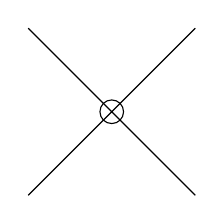
\begin{tikzpicture}
          \begin{feynman}
            \vertex[crossed dot] (v) {};
            \vertex[above left = of v] (f1);
            \vertex[below left = of v] (f2);
            \vertex[above right = of v] (f3);
            \vertex[below right = of v] (f4);
            \diagram* {
              (f1) -- (v),
              (f2) -- (v),
              (v) -- (f3),
              (v) -- (f4), };
          \end{feynman}
        \end{tikzpicture}}
      = \shrink{
        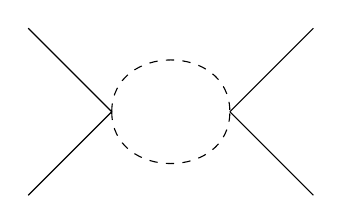
\begin{tikzpicture}
          \begin{feynman}
            \vertex (v1);
            \vertex[right = of v1] (v2);
            \vertex[above left = of v1] (f1);
            \vertex[below left = of v1] (f2);
            \vertex[above right = of v2] (f3);
            \vertex[below right = of v2] (f4);
            \diagram* {
              (f1) -- (v1) --[half left, scalar] (v2) -- (f3),
              (f2) -- (v1) --[half right, scalar] (v2) -- (f4), };
          \end{feynman}
        \end{tikzpicture}},
      \tag{30}
    \end{align}
    which can be expanded and solved explicitly for the counter-terms
    to find
    \begin{align}
      \widetilde G^{rs}_{r''s''}
      = \sum_{\ell,m,r',s'} \f{K_{\ell m}^2}{K E_{\ell m}}
      G^{rs}_{r's'} G^{r's'}_{r''s''}.
      \tag{31}
    \end{align}
    In terms of ordinary coupling constants, the counter-term diagram
    in (24) is therefore
    \begin{align}
      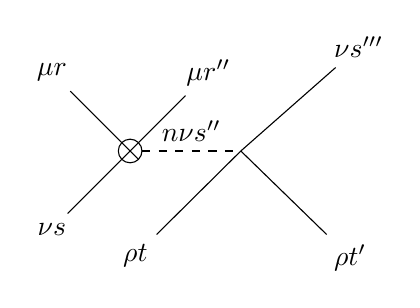
\begin{tikzpicture}
        \begin{feynman}
          \vertex[crossed dot] (v1) {};
          \vertex[above left = 4em of v1] (f1) {$\mu r$};
          \vertex[below left = 4em of v1] (f2) {$\nu s$};
          \vertex[right = 4em of v1] (v2);
          \vertex[above right = 4em of v1] (f3) {$\mu r''$};
          \vertex[below left = of v2] (f4) {$\rho t$};
          \vertex[below right = of v2] (f5) {$\rho t'$};
          \vertex[above right = of v2] (f6) {$\nu s'''$};
          \diagram* {
            (f1) -- (v1) -- (f3),
            (f2) -- (v1)
            --[scalar, edge label=$n\nu s''$] (v2),
            (f4) -- (v2) -- (f5),
            (v2) -- (f6), };
        \end{feynman}
      \end{tikzpicture}
      = \sum_{\ell,m,r',s'}
      \f{K_{\ell m}^2 K_n^2}{K E_{\ell m} E_n}
      G^{rs}_{r's'} G^{r's'}_{r''s''} G^{s''t}_{s'''t'}
      \c_{\mu r''}^\dag \c_{\nu s'''}^\dag \c_{\rho t'}^\dag
      \c_{\rho t} \c_{\nu s} \c_{\mu r}.
      \tag{32}
    \end{align}
    Altogether, the contribution to the third-order three-body
    interaction Hamiltonian from loop diagrams of the form in (23) and
    counter-term diagrams of the form in (24) is
    \begin{multline}
      \shrink{
        \begin{tikzpicture}
          \begin{feynman}
            \vertex (v1);
            \vertex[right = of v1] (v2);
            \vertex[below right = of v2] (v3);
            \vertex[above left = of v1] (f1);
            \vertex[below left = of v1] (f2);
            \vertex[below left = of v3] (f3);
            \vertex[above right = of v2] (f4);
            \vertex[above right = of v3] (f5);
            \vertex[below right = of v3] (f6);
            \diagram* {
              (f1) -- (v1) --[half left, scalar] (v2) -- (f4),
              (f2) -- (v1) --[half right, scalar] (v2)
              --[scalar] (v3) -- (f5),
              (f3) -- (v3) -- (f6), };
          \end{feynman}
        \end{tikzpicture}}
        - \shrink{
        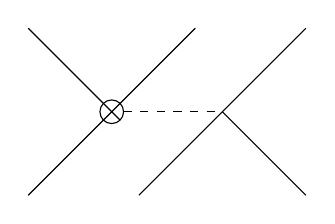
\begin{tikzpicture}
          \begin{feynman}
            \vertex[crossed dot] (v1) {};
            \vertex[right = 4em of v1] (v2);
            \vertex[above left = of v1] (f1);
            \vertex[below left = of v1] (f2);
            \vertex[above right = of v1] (f3);
            \vertex[below left = of v2] (f4);
            \vertex[below right = of v2] (f5);
            \vertex[above right = of v2] (f6);
            \diagram* {
              (f1) -- (v1) -- (f3),
              (f2) -- (v1) --[scalar] (v2),
              (f4) -- (v2) -- (f5),
              (v2) -- (f6), };
          \end{feynman}
        \end{tikzpicture}}
      - \f12 \shrink{
        \begin{tikzpicture}
          \begin{feynman}
            \vertex (v1);
            \vertex[right = of v1] (v2);
            \vertex[below right = of v2] (v3);
            \vertex[above left = of v1] (f1);
            \vertex[below left = of v1] (f2);
            \vertex[below left = of v3] (f3);
            \vertex[above right = of v2] (f4);
            \vertex[above right = of v3] (f5);
            \vertex[below right = of v3] (f6);
            \diagram* {
              (f1) -- (v1) --[half left, scalar] (v2) -- (f4),
              (f2) -- (v1) --[half right, scalar] (v2)
              -- (v3) -- (f5),
              (f3) -- (v3) -- (f6), };
          \end{feynman}
        \end{tikzpicture}}
      - \f12 \shrink{
        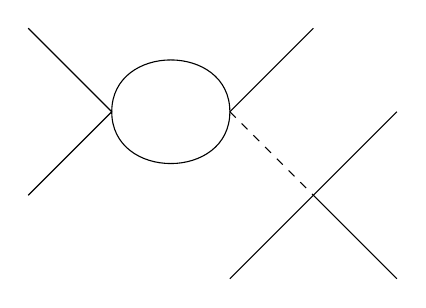
\begin{tikzpicture}
          \begin{feynman}
            \vertex (v1);
            \vertex[right = of v1] (v2);
            \vertex[below right = of v2] (v3);
            \vertex[above left = of v1] (f1);
            \vertex[below left = of v1] (f2);
            \vertex[below left = of v3] (f3);
            \vertex[above right = of v2] (f4);
            \vertex[above right = of v3] (f5);
            \vertex[below right = of v3] (f6);
            \diagram* {
              (f1) -- (v1) --[half left] (v2) -- (f4),
              (f2) -- (v1) --[half right] (v2)
              --[scalar] (v3) -- (f5),
              (f3) -- (v3) -- (f6), };
          \end{feynman}
        \end{tikzpicture}} \\
      = \p{\alpha_{3,2}^{(3)} - \f12\alpha_{4,3}^{(3)}
        - \f12\alpha_5^{(3)}}
      \H_{3,2}^{(3)},
      \tag{33}
    \end{multline}
    where
    \begin{align}
      \alpha_{3,2}^{(3)}
      \equiv \sum_{\substack{\ell+m>0\\n>0}}
      \f{K_{\ell m} K_n}{E_{\ell m} E_n}
      \p{K^{\ell m}_n - \f{K_{\ell m} K_n}{K}},
      &&
      \alpha_{4,3}^{(3)}
      \equiv K \sum_{m+n>0} \f{K_{mn}^2}{E_{mn}^2},
      \tag{34}
    \end{align}
    and
    \begin{align}
      \H_{3,2}^{(3)} \equiv \sum_{\abs{\set{\mu,\nu,\rho}}=3}
      G^{rs}_{r's'} G^{r's'}_{r''s''} G^{s''t}_{s'''t'}
      \c_{\mu r''}^\dag \c_{\nu s'''}^\dag \c_{\rho t'}^\dag
      \c_{\rho t} \c_{\nu s} \c_{\mu r}.
      \tag{35}
    \end{align}
    An equal contribution comes from the mirror images of these
    diagrams, such that the net third-order three-body interaction
    Hamiltonian is
    \begin{align}
      H_3^{(3)} = \p{\alpha_{3,1}^{(3)} - \alpha_5^{(3)}} \H_{3,1}^{(3)}
      + \p{2\alpha_{3,2}^{(3)} - \alpha_{4,3}^{(3)} - \alpha_5^{(3)}}
      \H_{3,2}^{(3)}.
      \tag{36}
    \end{align}
    Note that the aforementioned divergence and its cancellation are
    buried in $\alpha_{3,2}^{(3)}$.  Formally, this factor is
    calculated by imposing an ultraviolet cutoff $\Lambda$ for the
    maximum values of motional state indices $\ell,m,n$, and then
    taking the limit $\Lambda\to\infty$.  This procedure ensures that
    $\alpha_{3,2}^{(3)}$ always remains finite.}


\item To reflect the changes above, in the last appendix (G) we have
  replaced all instances of \red{$\alpha_3^{(1)}$} with
  \green{$\alpha_{3,1}^{(3)}$}, and the replaced prefactor
  \red{$-\p{\alpha_{4,3}^{(3)}+\alpha_5^{(3)}}$} by
  \green{$+ \p{2\alpha_{3,2}^{(3)} - \alpha_{4,3}^{(3)} -
      \alpha_5^{(3)}}$}.


\item In addition, we have rearranged some of the text in section
  III.E in order for this section to have a structure similar to that
  of section III.D.  To this end, we have replaced the following text
  (page 21, line 49):

  \red{Observing that the diagrams of the form in (36) are equal to
    their mirror image, the positive contributions to the third-order
    four-body interaction Hamiltonian are
    \begin{align}
      \shrink{
        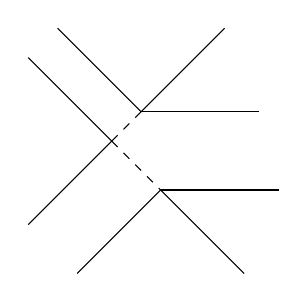
\begin{tikzpicture}
          \begin{feynman}
            \vertex (v1);
            \vertex[above right = 1.5em of v1] (v2);
            \vertex[below right = 2.5em of v1] (v3);
            \vertex[above left = of v1] (f1);
            \vertex[below left = of v1] (f2);
            \vertex[above left = of v2] (f3);
            \vertex[below left = of v3] (f4);
            \vertex[above right = of v2] (f5);
            \vertex[right = of v2] (f6);
            \vertex[right = of v3] (f7);
            \vertex[below right = of v3] (f8);
            \diagram* {
              (f1) -- (v1) --[scalar] (v2) -- (f6),
              (f2) -- (v1) --[scalar] (v3) -- (f7),
              (f3) -- (v2) -- (f5),
              (f4) -- (v3) -- (f8),
            };
          \end{feynman}
        \end{tikzpicture}}
      + \shrink{
        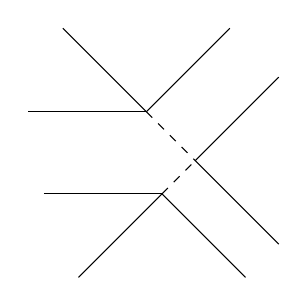
\begin{tikzpicture}
          \begin{feynman}
            \vertex (v1);
            \vertex[below right = 2.5em of v1] (v3);
            \vertex[below left = 1.7em of v3] (v2);
            \vertex[above left = of v1] (f1);
            \vertex[left = of v1] (f2);
            \vertex[left = of v2] (f3);
            \vertex[below left = of v2] (f4);
            \vertex[above right = of v1] (f5);
            \vertex[above right = of v3] (f6);
            \vertex[below right = of v3] (f7);
            \vertex[below right = of v2] (f8);
            \diagram* {
              (f1) -- (v1) -- (f5),
              (f2) -- (v1) --[scalar] (v3) -- (f6),
              (f3) -- (v2) --[scalar] (v3) -- (f7),
              (f4) -- (v2) -- (f8), };
          \end{feynman}
        \end{tikzpicture}}
      + \shrink{
        \begin{tikzpicture}
          \begin{feynman}
            \vertex (v1);
            \vertex[below right = of v1] (v2);
            \vertex[below right = of v2] (v3);
            \vertex[above left = of v1] (f1);
            \vertex[below left = of v1] (f2);
            \vertex[below left = of v2] (f3);
            \vertex[below left = of v3] (f4);
            \vertex[above right = of v1] (f5);
            \vertex[above right = of v2] (f6);
            \vertex[above right = of v3] (f7);
            \vertex[below right = of v3] (f8);
            \diagram* {
              (f1) -- (v1) -- (f5),
              (f2) -- (v1) -- (f5),
              (v1) --[scalar] (v2) --[scalar] (v3) -- (f8),
              (f3) -- (v2) -- (f6),
              (f4) -- (v3) -- (f7),
            };
          \end{feynman}
        \end{tikzpicture}}
      = 2 \shrink{
        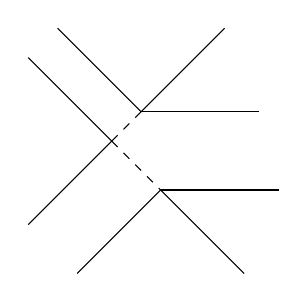
\begin{tikzpicture}
          \begin{feynman}
            \vertex (v1);
            \vertex[above right = 1.5em of v1] (v2);
            \vertex[below right = 2.5em of v1] (v3);
            \vertex[above left = of v1] (f1);
            \vertex[below left = of v1] (f2);
            \vertex[above left = of v2] (f3);
            \vertex[below left = of v3] (f4);
            \vertex[above right = of v2] (f5);
            \vertex[right = of v2] (f6);
            \vertex[right = of v3] (f7);
            \vertex[below right = of v3] (f8);
            \diagram* {
              (f1) -- (v1) --[scalar] (v2) -- (f6),
              (f2) -- (v1) --[scalar] (v3) -- (f7),
              (f3) -- (v2) -- (f5),
              (f4) -- (v3) -- (f8),
            };
          \end{feynman}
        \end{tikzpicture}}
      + \shrink{
        \begin{tikzpicture}
          \begin{feynman}
            \vertex (v1);
            \vertex[below right = of v1] (v2);
            \vertex[below right = of v2] (v3);
            \vertex[above left = of v1] (f1);
            \vertex[below left = of v1] (f2);
            \vertex[below left = of v2] (f3);
            \vertex[below left = of v3] (f4);
            \vertex[above right = of v1] (f5);
            \vertex[above right = of v2] (f6);
            \vertex[above right = of v3] (f7);
            \vertex[below right = of v3] (f8);
            \diagram* {
              (f1) -- (v1) -- (f5),
              (f2) -- (v1) -- (f5),
              (v1) --[scalar] (v2) --[scalar] (v3) -- (f8),
              (f3) -- (v2) -- (f6),
              (f4) -- (v3) -- (f7),
            };
          \end{feynman}
        \end{tikzpicture}},
      \tag{38}
    \end{align}
    while the negative contributions are
    \begin{multline}
      \f12 \shrink{
        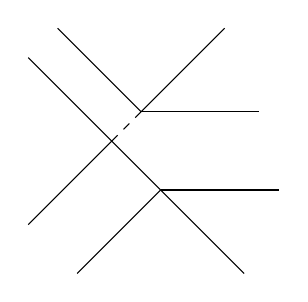
\begin{tikzpicture}
          \begin{feynman}
            \vertex (v1);
            \vertex[above right = 1.5em of v1] (v2);
            \vertex[below right = 2.5em of v1] (v3);
            \vertex[above left = of v1] (f1);
            \vertex[below left = of v1] (f2);
            \vertex[above left = of v2] (f3);
            \vertex[below left = of v3] (f4);
            \vertex[above right = of v2] (f5);
            \vertex[right = of v2] (f6);
            \vertex[right = of v3] (f7);
            \vertex[below right = of v3] (f8);
            \diagram* {
              (f1) -- (v1) --[scalar] (v2) -- (f6),
              (f2) -- (v1) -- (v3) -- (f7),
              (f3) -- (v2) -- (f5),
              (f4) -- (v3) -- (f8),
            };
          \end{feynman}
        \end{tikzpicture}}
      + \f12 \shrink{
        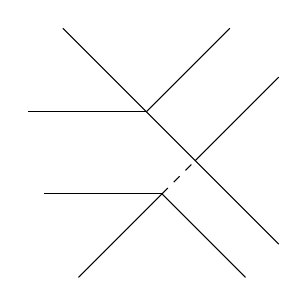
\begin{tikzpicture}
          \begin{feynman}
            \vertex (v1);
            \vertex[below right = 2.5em of v1] (v3);
            \vertex[below left = 1.7em of v3] (v2);
            \vertex[above left = of v1] (f1);
            \vertex[left = of v1] (f2);
            \vertex[left = of v2] (f3);
            \vertex[below left = of v2] (f4);
            \vertex[above right = of v1] (f5);
            \vertex[above right = of v3] (f6);
            \vertex[below right = of v3] (f7);
            \vertex[below right = of v2] (f8);
            \diagram* {
              (f1) -- (v1) -- (f5),
              (f2) -- (v1) -- (v3) -- (f6),
              (f3) -- (v2) --[scalar] (v3) -- (f7),
              (f4) -- (v2) -- (f8), };
          \end{feynman}
        \end{tikzpicture}}
      + \f12 \shrink{
        \begin{tikzpicture}
          \begin{feynman}
            \vertex (v1);
            \vertex[below right = of v1] (v2);
            \vertex[below right = of v2] (v3);
            \vertex[above left = of v1] (f1);
            \vertex[below left = of v1] (f2);
            \vertex[below left = of v2] (f3);
            \vertex[below left = of v3] (f4);
            \vertex[above right = of v1] (f5);
            \vertex[above right = of v2] (f6);
            \vertex[above right = of v3] (f7);
            \vertex[below right = of v3] (f8);
            \diagram* {
              (f1) -- (v1) -- (f5),
              (f2) -- (v1) -- (f5),
              (v1) --[scalar] (v2) -- (v3) -- (f8),
              (f3) -- (v2) -- (f6),
              (f4) -- (v3) -- (f7),
            };
          \end{feynman}
        \end{tikzpicture}}
      + \f12 \shrink{
        \begin{tikzpicture}
          \begin{feynman}
            \vertex (v1);
            \vertex[below right = of v1] (v2);
            \vertex[below right = of v2] (v3);
            \vertex[above left = of v1] (f1);
            \vertex[below left = of v1] (f2);
            \vertex[below left = of v2] (f3);
            \vertex[below left = of v3] (f4);
            \vertex[above right = of v1] (f5);
            \vertex[above right = of v2] (f6);
            \vertex[above right = of v3] (f7);
            \vertex[below right = of v3] (f8);
            \diagram* {
              (f1) -- (v1) -- (f5),
              (f2) -- (v1) -- (f5),
              (v1) -- (v2) --[scalar] (v3) -- (f8),
              (f3) -- (v2) -- (f6),
              (f4) -- (v3) -- (f7),
            };
          \end{feynman}
        \end{tikzpicture}} \\
      = \shrink{
        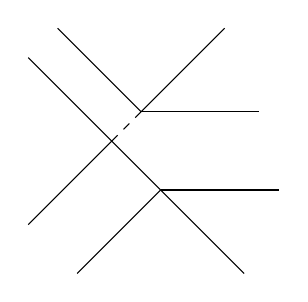
\begin{tikzpicture}
          \begin{feynman}
            \vertex (v1);
            \vertex[above right = 1.5em of v1] (v2);
            \vertex[below right = 2.5em of v1] (v3);
            \vertex[above left = of v1] (f1);
            \vertex[below left = of v1] (f2);
            \vertex[above left = of v2] (f3);
            \vertex[below left = of v3] (f4);
            \vertex[above right = of v2] (f5);
            \vertex[right = of v2] (f6);
            \vertex[right = of v3] (f7);
            \vertex[below right = of v3] (f8);
            \diagram* {
              (f1) -- (v1) --[scalar] (v2) -- (f6),
              (f2) -- (v1) -- (v3) -- (f7),
              (f3) -- (v2) -- (f5),
              (f4) -- (v3) -- (f8),
            };
          \end{feynman}
        \end{tikzpicture}}
      + \shrink{
        \begin{tikzpicture}
          \begin{feynman}
            \vertex (v1);
            \vertex[below right = of v1] (v2);
            \vertex[below right = of v2] (v3);
            \vertex[above left = of v1] (f1);
            \vertex[below left = of v1] (f2);
            \vertex[below left = of v2] (f3);
            \vertex[below left = of v3] (f4);
            \vertex[above right = of v1] (f5);
            \vertex[above right = of v2] (f6);
            \vertex[above right = of v3] (f7);
            \vertex[below right = of v3] (f8);
            \diagram* {
              (f1) -- (v1) -- (f5),
              (f2) -- (v1) -- (f5),
              (v1) --[scalar] (v2) -- (v3) -- (f8),
              (f3) -- (v2) -- (f6),
              (f4) -- (v3) -- (f7),
            };
          \end{feynman}
        \end{tikzpicture}},
      \tag{39}
    \end{multline}
    such that the net third-order four-body interaction Hamiltonian is
    \begin{align}
      H_4^{(3)} &= 2 \shrink{
        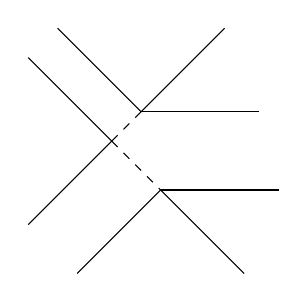
\begin{tikzpicture}
          \begin{feynman}
            \vertex (v1);
            \vertex[above right = 1.5em of v1] (v2);
            \vertex[below right = 2.5em of v1] (v3);
            \vertex[above left = of v1] (f1);
            \vertex[below left = of v1] (f2);
            \vertex[above left = of v2] (f3);
            \vertex[below left = of v3] (f4);
            \vertex[above right = of v2] (f5);
            \vertex[right = of v2] (f6);
            \vertex[right = of v3] (f7);
            \vertex[below right = of v3] (f8);
            \diagram* {
              (f1) -- (v1) --[scalar] (v2) -- (f6),
              (f2) -- (v1) --[scalar] (v3) -- (f7),
              (f3) -- (v2) -- (f5),
              (f4) -- (v3) -- (f8),
            };
          \end{feynman}
        \end{tikzpicture}}
      - \shrink{
        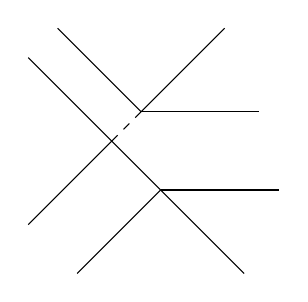
\begin{tikzpicture}
          \begin{feynman}
            \vertex (v1);
            \vertex[above right = 1.5em of v1] (v2);
            \vertex[below right = 2.5em of v1] (v3);
            \vertex[above left = of v1] (f1);
            \vertex[below left = of v1] (f2);
            \vertex[above left = of v2] (f3);
            \vertex[below left = of v3] (f4);
            \vertex[above right = of v2] (f5);
            \vertex[right = of v2] (f6);
            \vertex[right = of v3] (f7);
            \vertex[below right = of v3] (f8);
            \diagram* {
              (f1) -- (v1) --[scalar] (v2) -- (f6),
              (f2) -- (v1) -- (v3) -- (f7),
              (f3) -- (v2) -- (f5),
              (f4) -- (v3) -- (f8),
            };
          \end{feynman}
        \end{tikzpicture}}
      + \shrink{
        \begin{tikzpicture}
          \begin{feynman}
            \vertex (v1);
            \vertex[below right = of v1] (v2);
            \vertex[below right = of v2] (v3);
            \vertex[above left = of v1] (f1);
            \vertex[below left = of v1] (f2);
            \vertex[below left = of v2] (f3);
            \vertex[below left = of v3] (f4);
            \vertex[above right = of v1] (f5);
            \vertex[above right = of v2] (f6);
            \vertex[above right = of v3] (f7);
            \vertex[below right = of v3] (f8);
            \diagram* {
              (f1) -- (v1) -- (f5),
              (f2) -- (v1) -- (f5),
              (v1) --[scalar] (v2) --[scalar] (v3) -- (f8),
              (f3) -- (v2) -- (f6),
              (f4) -- (v3) -- (f7),
            };
          \end{feynman}
        \end{tikzpicture}}
      - \shrink{
        \begin{tikzpicture}
          \begin{feynman}
            \vertex (v1);
            \vertex[below right = of v1] (v2);
            \vertex[below right = of v2] (v3);
            \vertex[above left = of v1] (f1);
            \vertex[below left = of v1] (f2);
            \vertex[below left = of v2] (f3);
            \vertex[below left = of v3] (f4);
            \vertex[above right = of v1] (f5);
            \vertex[above right = of v2] (f6);
            \vertex[above right = of v3] (f7);
            \vertex[below right = of v3] (f8);
            \diagram* {
              (f1) -- (v1) -- (f5),
              (f2) -- (v1) -- (f5),
              (v1) --[scalar] (v2) -- (v3) -- (f8),
              (f3) -- (v2) -- (f6),
              (f4) -- (v3) -- (f7),
            };
          \end{feynman}
        \end{tikzpicture}} \nonumber \\
      &= \p{2\alpha_{4,1}^{(3)} - \alpha_5^{(3)}} \H_{4,1}^{(3)}
      + \p{\alpha_{4,2}^{(3)} - \alpha_5^{(3)}} \H_{4,2}^{(3)},
      \tag{40}
    \end{align}
    where
    \begin{align}
      \alpha_{4,1}^{(3)}
      \equiv \sum_{\substack{m\ge0\\n>0}} \f{K_{mn} K_m K_n}{E_{mn} E_n},
      &&
      \alpha_{4,2}^{(3)}
      \equiv \sum_{m,n>0} \f{K_m K^m_n K_n}{E_m E_n},
      &&
      \alpha_5^{(3)}
      \equiv  K \sum_{n>0} \f{K_n^2}{E_n^2},
      \tag{41}
    \end{align}
    \begin{align}
      \H_{4,1}^{(3)}
      \equiv \sum_{\abs{\set{\mu,\nu,\rho,\sigma}}=4}
      G^{qr}_{q'r'} G^{q's}_{q''s'} G^{r't}_{r''t'}
      \c_{\mu q''}^\dag \c_{\nu r''}^\dag
      \c_{\rho s'}^\dag \c_{\sigma t'}^\dag
      \c_{\sigma t} \c_{\rho s} \c_{\nu r} \c_{\mu q},
      \tag{42}
    \end{align}
    \begin{align}
      \H_{4,2}^{(3)}
      \equiv \sum_{\abs{\set{\mu,\nu,\rho,\sigma}}=4}
      G^{qr}_{q'r'} G^{\mu q'\rho s}_{\mu'q''\rho's'} G^{q''t}_{q'''t'}
      \c_{\mu'q'''}^\dag \c_{\nu r'}^\dag
      \c_{\rho's'}^\dag \c_{\sigma t'}^\dag
      \c_{\sigma t} \c_{\rho s} \c_{\nu r} \c_{\mu q}.
      \tag{43}
    \end{align}}

  by:

  \green{The contribution to the third-order four-body interaction
    Hamiltonian from diagrams of the form in (37) is
    \begin{align}
      \shrink{
        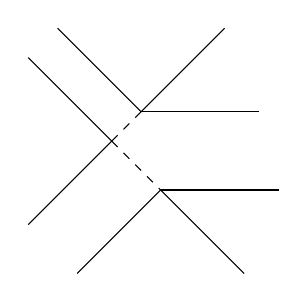
\begin{tikzpicture}
          \begin{feynman}
            \vertex (v1);
            \vertex[above right = 1.5em of v1] (v2);
            \vertex[below right = 2.5em of v1] (v3);
            \vertex[above left = of v1] (f1);
            \vertex[below left = of v1] (f2);
            \vertex[above left = of v2] (f3);
            \vertex[below left = of v3] (f4);
            \vertex[above right = of v2] (f5);
            \vertex[right = of v2] (f6);
            \vertex[right = of v3] (f7);
            \vertex[below right = of v3] (f8);
            \diagram* {
              (f1) -- (v1) --[scalar] (v2) -- (f6),
              (f2) -- (v1) --[scalar] (v3) -- (f7),
              (f3) -- (v2) -- (f5),
              (f4) -- (v3) -- (f8),
            };
          \end{feynman}
        \end{tikzpicture}}
      - \f12 \shrink{
        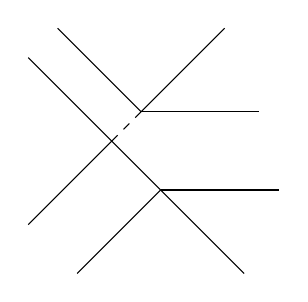
\begin{tikzpicture}
          \begin{feynman}
            \vertex (v1);
            \vertex[above right = 1.5em of v1] (v2);
            \vertex[below right = 2.5em of v1] (v3);
            \vertex[above left = of v1] (f1);
            \vertex[below left = of v1] (f2);
            \vertex[above left = of v2] (f3);
            \vertex[below left = of v3] (f4);
            \vertex[above right = of v2] (f5);
            \vertex[right = of v2] (f6);
            \vertex[right = of v3] (f7);
            \vertex[below right = of v3] (f8);
            \diagram* {
              (f1) -- (v1) --[scalar] (v2) -- (f6),
              (f2) -- (v1) -- (v3) -- (f7),
              (f3) -- (v2) -- (f5),
              (f4) -- (v3) -- (f8),
            };
          \end{feynman}
        \end{tikzpicture}}
      = \p{\alpha_{4,1}^{(3)} - \f12\alpha_5^{(3)}} \H_{4,1},
      \tag{40}
    \end{align}
    where
    \begin{align}
      \alpha_{4,1}^{(3)}
      \equiv \sum_{\substack{m\ge0\\n>0}} \f{K_{mn} K_m K_n}{E_{mn} E_n},
      \tag{41}
    \end{align}
    and
    \begin{align}
      \H_{4,1}^{(3)}
      \equiv \sum_{\abs{\set{\mu,\nu,\rho,\sigma}}=4}
      G^{qr}_{q'r'} G^{q's}_{q''s'} G^{r't}_{r''t'}
      \c_{\mu q''}^\dag \c_{\nu r''}^\dag
      \c_{\rho s'}^\dag \c_{\sigma t'}^\dag
      \c_{\sigma t} \c_{\rho s} \c_{\nu r} \c_{\mu q}.
      \tag{42}
    \end{align}
    An equal contribution comes from the mirror images of these
    diagrams.  The contribution from diagrams of the form in (38),
    meanwhile, is
    \begin{align}
      \shrink{
        \begin{tikzpicture}
          \begin{feynman}
            \vertex (v1);
            \vertex[below right = of v1] (v2);
            \vertex[below right = of v2] (v3);
            \vertex[above left = of v1] (f1);
            \vertex[below left = of v1] (f2);
            \vertex[below left = of v2] (f3);
            \vertex[below left = of v3] (f4);
            \vertex[above right = of v1] (f5);
            \vertex[above right = of v2] (f6);
            \vertex[above right = of v3] (f7);
            \vertex[below right = of v3] (f8);
            \diagram* {
              (f1) -- (v1) -- (f5),
              (f2) -- (v1) -- (f5),
              (v1) --[scalar] (v2) --[scalar] (v3) -- (f8),
              (f3) -- (v2) -- (f6),
              (f4) -- (v3) -- (f7),
            };
          \end{feynman}
        \end{tikzpicture}}
      - \f12 \shrink{
        \begin{tikzpicture}
          \begin{feynman}
            \vertex (v1);
            \vertex[below right = of v1] (v2);
            \vertex[below right = of v2] (v3);
            \vertex[above left = of v1] (f1);
            \vertex[below left = of v1] (f2);
            \vertex[below left = of v2] (f3);
            \vertex[below left = of v3] (f4);
            \vertex[above right = of v1] (f5);
            \vertex[above right = of v2] (f6);
            \vertex[above right = of v3] (f7);
            \vertex[below right = of v3] (f8);
            \diagram* {
              (f1) -- (v1) -- (f5),
              (f2) -- (v1) -- (f5),
              (v1) --[scalar] (v2) -- (v3) -- (f8),
              (f3) -- (v2) -- (f6),
              (f4) -- (v3) -- (f7),
            };
          \end{feynman}
        \end{tikzpicture}}
      - \f12 \shrink{
        \begin{tikzpicture}
          \begin{feynman}
            \vertex (v1);
            \vertex[below right = of v1] (v2);
            \vertex[below right = of v2] (v3);
            \vertex[above left = of v1] (f1);
            \vertex[below left = of v1] (f2);
            \vertex[below left = of v2] (f3);
            \vertex[below left = of v3] (f4);
            \vertex[above right = of v1] (f5);
            \vertex[above right = of v2] (f6);
            \vertex[above right = of v3] (f7);
            \vertex[below right = of v3] (f8);
            \diagram* {
              (f1) -- (v1) -- (f5),
              (f2) -- (v1) -- (f5),
              (v1) -- (v2) --[scalar] (v3) -- (f8),
              (f3) -- (v2) -- (f6),
              (f4) -- (v3) -- (f7),
            };
          \end{feynman}
        \end{tikzpicture}}
      = \p{\alpha_{4,2}^{(3)} - \alpha_5^{(3)}} \H_{4,2},
      \tag{43}
    \end{align}
    where
    \begin{align}
      \alpha_{4,2}^{(3)}
      \equiv \sum_{m,n>0} \f{K_m K^m_n K_n}{E_m E_n},
      \tag{44}
    \end{align}
    and
    \begin{align}
      \H_{4,2}^{(3)}
      \equiv \sum_{\abs{\set{\mu,\nu,\rho,\sigma}}=4}
      G^{qr}_{q'r'} G^{\mu q'\rho s}_{\mu'q''\rho's'} G^{q''t}_{q'''t'}
      \c_{\mu'q'''}^\dag \c_{\nu r'}^\dag
      \c_{\rho's'}^\dag \c_{\sigma t'}^\dag
      \c_{\sigma t} \c_{\rho s} \c_{\nu r} \c_{\mu q}.
      \tag{45}
    \end{align}
    The net third-order four-body interaction Hamiltonian is therefore
    \begin{align}
      H_4^{(3)}
      = \p{2\alpha_{4,1}^{(3)} - \alpha_5^{(3)}} \H_{4,1}^{(3)}
      + \p{\alpha_{4,2}^{(3)} - \alpha_5^{(3)}} \H_{4,2}^{(3)}.
      \tag{46}
    \end{align}}

\item Finally, we have re-computed all of our numerical results, and
  updated figures 3, 4, and 5 accordingly.  The changes to these
  figures are small enough as to be nearly imperceptible to the eye,
  and therefore do not affect any of the discussions or conclusions in
  our manuscript.

\end{enumerate}

\end{document}